%File: formatting-instructions-latex-2023.tex
%release 2023.0
\documentclass[letterpaper]{article} % DO NOT CHANGE THIS

\usepackage{aaai23}  % DO NOT CHANGE THIS
\usepackage{times}  % DO NOT CHANGE THIS
\usepackage{helvet}  % DO NOT CHANGE THIS
\usepackage{courier}  % DO NOT CHANGE THIS
\usepackage[hyphens]{url}  % DO NOT CHANGE THIS
\usepackage{graphicx} % DO NOT CHANGE THIS
\urlstyle{rm} % DO NOT CHANGE THIS
\def\UrlFont{\rm}  % DO NOT CHANGE THIS
\usepackage{natbib}  % DO NOT CHANGE THIS AND DO NOT ADD ANY OPTIONS TO IT
\usepackage{caption} % DO NOT CHANGE THIS AND DO NOT ADD ANY OPTIONS TO IT
\frenchspacing  % DO NOT CHANGE THIS
\setlength{\pdfpagewidth}{8.5in}  % DO NOT CHANGE THIS
\setlength{\pdfpageheight}{11in}  % DO NOT CHANGE THIS
\usepackage{csvsimple}
% \usepackage{datatool}  
\usepackage{booktabs}
%
% These are recommended to typeset algorithms but not required. See the subsubsection on algorithms. Remove them if you don't have algorithms in your paper.
\usepackage{algorithm}
\usepackage{algorithmic}

\pdfinfo{
/TemplateVersion (2023.1)
}

%
% These are are recommended to typeset listings but not required. See the subsubsection on listing. Remove this block if you don't have listings in your paper.
\usepackage{newfloat}
\usepackage{listings}
\DeclareCaptionStyle{ruled}{labelfont=normalfont,labelsep=colon,strut=off} % DO NOT CHANGE THIS
\lstset{%
	basicstyle={\footnotesize\ttfamily},% footnotesize acceptable for monospace
	numbers=left,numberstyle=\footnotesize,xleftmargin=2em,% show line numbers, remove this entire line if you don't want the numbers.
	aboveskip=0pt,belowskip=0pt,%
	showstringspaces=false,tabsize=2,breaklines=true}
\floatstyle{ruled}
\newfloat{listing}{tb}{lst}{}
\floatname{listing}{Listing}

% DISALLOWED PACKAGES
% \usepackage{authblk} -- This package is specifically forbidden
% \usepackage{balance} -- This package is specifically forbidden
% \usepackage{color (if used in text)
% \usepackage{CJK} -- This package is specifically forbidden
% \usepackage{float} -- This package is specifically forbidden
% \usepackage{flushend} -- This package is specifically forbidden
% \usepackage{fontenc} -- This package is specifically forbidden
% \usepackage{fullpage} -- This package is specifically forbidden
% \usepackage{geometry} -- This package is specifically forbidden
% \usepackage{grffile} -- This package is specifically forbidden
% \usepackage{hyperref} -- This package is specifically forbidden
% \usepackage{navigator} -- This package is specifically forbidden
% (or any other package that embeds links such as navigator or hyperref)
% \indentfirst} -- This package is specifically forbidden
% \layout} -- This package is specifically forbidden
% \multicol} -- This package is specifically forbidden
% \nameref} -- This package is specifically forbidden
% \usepackage{savetrees} -- This package is specifically forbidden
% \usepackage{setspace} -- This package is specifically forbidden
% \usepackage{stfloats} -- This package is specifically forbidden
% \usepackage{tabu} -- This package is specifically forbidden
% \usepackage{titlesec} -- This package is specifically forbidden
% \usepackage{tocbibind} -- This package is specifically forbidden
% \usepackage{ulem} -- This package is specifically forbidden
% \usepackage{wrapfig} -- This package is specifically forbidden
% DISALLOWED COMMANDS
% \nocopyright -- Your paper will not be published if you use this command
% \addtolength -- This command may not be used
% \balance -- This command may not be used
% \baselinestretch -- Your paper will not be published if you use this command
% \clearpage -- No page breaks of any kind may be used for the final version of your paper
% \columnsep -- This command may not be used
% \newpage -- No page breaks of any kind may be used for the final version of your paper
% \pagebreak -- No page breaks of any kind may be used for the final version of your paperr
% \pagestyle -- This command may not be used
% \tiny -- This is not an acceptable font size.
% \vspace{- -- No negative value may be used in proximity of a caption, figure, table, section, subsection, subsubsection, or reference
% \vskip{- -- No negative value may be used to alter spacing above or below a caption, figure, table, section, subsection, subsubsection, or reference

\setcounter{secnumdepth}{0} %May be changed to 1 or 2 if section numbers are desired.

% The file aaai23.sty is the style file for AAAI Press
% proceedings, working notes, and technical reports.
%

% Title

% Your title must be in mixed case, not sentence case.
% That means all verbs (including short verbs like be, is, using,and go),
% nouns, adverbs, adjectives should be capitalized, including both words in hyphenated terms, while
% articles, conjunctions, and prepositions are lower case unless they
% directly follow a colon or long dash
\title{BIOS 823 Final Project: Colorectal Cancer Histology Images Classification}
\author{
    %Authors
    % All authors must be in the same font size and format.
    Tengjie (TJ) Tang\textsuperscript{\rm 1}
}
\affiliations{
    %Afiliations
    \textsuperscript{\rm 1}Duke University Department of Statistical Science\\
    Durham, North Carolina 27705 USA\\
    tengjie.tang@duke.edu
%
% See more examples next
}

%Example, Single Author, ->> remove \iffalse,\fi and place them surrounding AAAI title to use it
\iffalse
\title{My Publication Title --- Single Author}
\author {
    Author Name
}
\affiliations{
    Affiliation\\
    Affiliation Line 2\\
    name@example.com
}
\fi


% REMOVE THIS: bibentry
% This is only needed to show inline citations in the guidelines document. You should not need it and can safely delete it.
\usepackage{bibentry}
% END REMOVE bibentry

\begin{document}

\maketitle

\begin{abstract}

In this project, I implement and compare the support vector machine, random forest, and three convolutional neural network architectures to classify textures in colorectal cancer histology. The results demonstrate that convolutional neural networks outperform the other two methods with higher classification accuracy for the image classification task. 

\end{abstract}

\section{Introduction}

Image classification is important for biomedical science studies. Medical imaging, including X-ray imaging, CT (Computed Tomography) Scanner, PET (Positron Emission Tomography), and MRI (Magnetic Resonance Imaging), is widely used in medical science in the modern world to aid internal body structures assessment and disease diagnosis and treatment \cite{Bajaj2018, ZHANG2019354, TchitoTchapga2021BiomedicalIC, hussain2022modern}. Precise medical imaging classification can help medical people to differentiate between normal and abnormal individuals and provide better treatments \cite{9669323}. 

In the project, I explored several supervised learning methods, including two machine learning methods, support vector machine and random forest, and three deep learning convolution neural network architectures, and compared their performance on a biomedical image classification task.

\section{Data set}

The data set for this project is \texttt{colorectal\_histology} \cite{kather2016multi} data set from the \texttt{TensorFlow} \cite{tensorflow2015-whitepaper} library. The data set has 5,000 histological images of human colorectal cancer. Each image is 150 x 150 x 3 RGB of one of eight tissue categories. The eight classes are tumor, stroma, complex, lympho, debris, mucosa, adipose, and empty. Figure~\ref{fig1} shows examples of images for each class with corresponding labels and class memberships.

\begin{figure}[t]
\centering
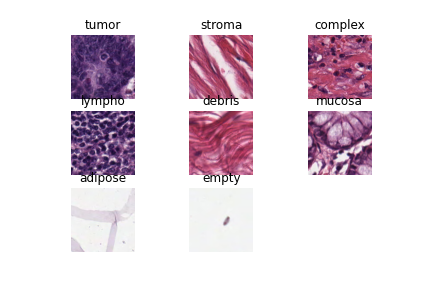
\includegraphics[width=0.9\columnwidth]{figures/intro.png} 
\caption{Visualization of sample images and corresponding labels}
\label{fig1}
\end{figure}

Images are scaled before applying the proposed methods so that pixels range between 0 and 1. Scaling can also help the learning process be much faster. 

\section{Methods}

\subsection{Support Vector Machine}

A support vector machine (SVM) \cite{boser1992training} is a supervised machine learning method for classification and regression analysis that maximizes the margin between the training data points and the hyperplane. The hyperplane is $p-1$ dimensional decision boundary for the linear SVM, where $p$ is the dimension of the feature space. 

The SVM is a linear classifier in its base form, but it can also incorporate kernels to allow non-linear decision boundaries. The radial basis function (RBF) kernel is a commonly used SVM kernel. However, the SVM is defined only for binary classifications. Therefore, we need to consider multiclass SVM as an extension for our data analysis. In \texttt{scikit-learn} \cite{scikit-learn}, the multiclass SVM is handled according to a one-versus-one approach. Specifically, $K(K-1)/2$ pairwise binary classifiers are fit, where $K$ is the total number of classes, and the class for a given data point (image) is the class that wins the most pairwise comparisons.

The SVM is appealing because it is a robust classifier and allows non-linear kernel and regularization. It has also shown good performance on image classification tasks \cite{7930302}.

\subsection{Random Forest}

Random forests (RF) \cite{breiman2001random} is another popular machine learning method, which can also be used for classification and regression analysis. RF is an ensemble learning method that builds upon decision trees. And a decision tree is a tree-based machine learning approach built by the Classification and Regression Trees (CART) algorithm \cite{leo1984classification}. CART selects the predictors for splitting and thresholds with the objective of minimizing misclassification errors at each split. CART is a greedy algorithm and gives the tree classifier high variance. RF controls the variance by building multiple trees on bootstrapped sub-datasets and averaging them. It also selects only a subset of predictors as the splitting candidates at each split. When making predictions, RF passes the new data point (image) to all trees, and the class that wins the most votes would be the class membership for that image.

\subsection{Convolutional Neural Network}

A convolutional neural network (CNN) is a deep learning method designed to extract relevant features directly from pixel images and is shown to have promising performance for image pattern recognition over other methods \cite{726791, VALUEVA2020232}. 

CNN architectures consist of the image input, convolutional (Conv) layers, max-pooling layers, fully connected layers (dense layers), and the softmax layer.
Here, I propose three CNN architectures with different numbers of Conv layers and dense layers:
\begin{itemize}
    \item 1 Conv layer  +  1 dense layer
    \item 3 Conv layers + 2 dense layers
    \item 5 Conv layers + 3 dense layers.
\end{itemize}

I trained the model in 500 epochs for all three CNN architectures, and early stopping was used. For this classification task, I used ReLU as the activation function, the sparse categorical crossentropy as the loss function, and the Adam algorithm as the optimizer with a learning rate of 0.0001. 


\begin{table}[t]
\centering
\resizebox{.95\columnwidth}{!}{
\begin{tabular}{ l l l l l }%
        \toprule Algorithm & Hyperparameters & Range & Best & Description \\
        \midrule
        \csvreader[late after line=\\,head to column
        names]{tables/hyperparameters.csv}{}%
        {\Algorithm & \Hyperparameters & \Range & \Best & \Description}%
        \bottomrule
    \end{tabular}}
\caption{Hyperparameters tuning for random forest and support vector machine and hyperparameters for the final model}
\label{hp}
\end{table}

\section{Results}

Machine learning and deep learning methods can suffer from overfitting problems. In particular, a model can perform exceptionally well on a training set but poorly on external data sets. I performed hyperparameter tuning for RF and SVM to mitigate model overfitting. Specifically, I shuffled the whole data set and split it into training (60\%), validation (20\%), and test (20\%) sets and then considered grid search to find the optimal combinations of hyperparameters that produce the best validation accuracy for RF and SVM. The validation set is used during the CNN training process to monitor the model's sparse categorical crossentropy validation loss at each epoch. Additionally, I added ``dropout'' to each CNN, a regularization technique that randomly ignores each hidden unit with a probability of 0.5, to avoid overfitting \cite{hinton2012improving}. 



Table~\ref{hp} shows the hyperparameter tuning and hyperparameters for the final model. For RF, the number of trees in the forest is 1,000, and the maximum depth of the tree is 100. The RBF kernel is used for the SVM, and the regularization parameter is 10. Figure~\ref{fig2} shows the training and validation loss curves for all three CNN architectures. We can see that the 3 Conv layers and 5 Conv layers CNN have the lowest validation loss at the end. Even though there are still overfitting issues, it is acceptable to use the 3 Conv layers and 5 Conv layers CNN architectures for classifications.


\begin{figure}[t]
\centering
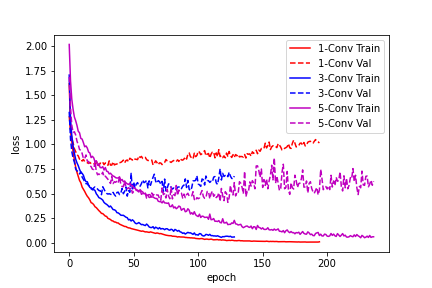
\includegraphics[width=0.9\columnwidth]{figures/cnn.png} 
\caption{Loss curve for three convolutional neural network architectures}
\label{fig2}
\end{figure}

The evaluation is performed on the test set. Table~\ref{tab2} reports the classification accuracy across all five proposed methods. From this, we can conclude that the 3 Conv layers and 5 Conv layers CNN has the best accuracy on the test set, and the 5 Conv layers CNN is slightly much better. The 1 Conv layer CNN has the worst performance and is worse than RF the SVM. 

Figure~\ref{cm} is the confusion matrix, which shows the classification performance for the best 5 Conv layers CNN model. It illustrates that the classification is very accurate across most of the classes. We can find that the model may misclassify stroma, debris, and complex tissue types. From Figure~\ref{fig1}, one of the reasons is probably because these tissues have similar colors and structures.

\begin{table}[t]
\centering
%\resizebox{.95\columnwidth}{!}{
\begin{tabular}{ l l l }%
        \toprule Model & Test Accuracy \\
        \midrule
        \csvreader[late after line=\\,head to column
        names]{tables/acc.csv}{}%
        {\Model & \Accuracy}%
        \bottomrule
    \end{tabular}
\caption{Test accuracy for all the models}
\label{tab2}
\end{table}



\begin{figure}[t]
\centering
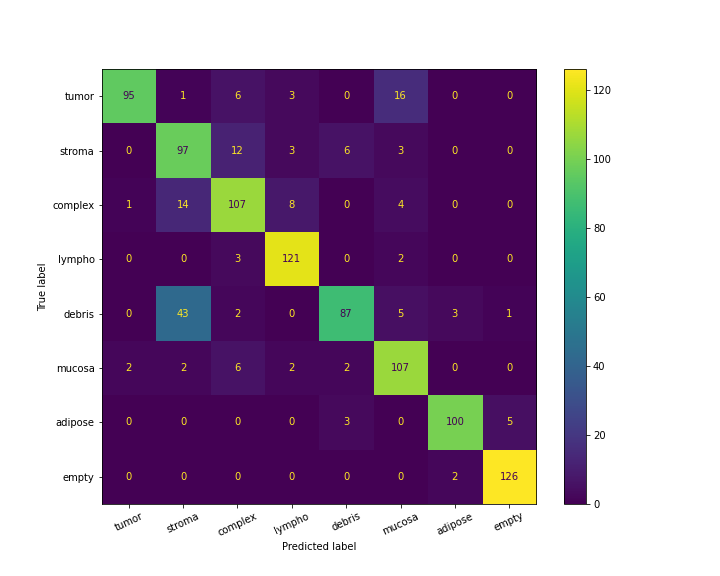
\includegraphics[width=0.9\columnwidth]{figures/confusion_matrix.png} 
\caption{Confusion matrix for the five convolutional layers convolutional neural network}
\label{cm}
\end{figure}

\section{Discussion and Conclusion}

In conclusion, among all CNN architectures, the 3 Conv layers and  5 Conv layers model has the best accuracy on the test sets. These two deep learning CNN performs better than the two machine learning methods (SVM and RF) in this image classification task. The 1 Conv layer CNN has the worst performance, which is because the model is too simple to learn the data set. Due to the limited computing power, I did not perform an exhaustive grid search and cross-validation parameters tuning for SVM and RF, and I did not perform fine-tuning for the three CNN architectures. Future studies could explore much deeper and different CNN architectures. We may also consider other useful techniques, including data augmentation and autoencoder. 



\appendix

% \paragraph{Website or online resource~\nocite{c:23}} Use the \texttt{@misc} class. Add the url in the \texttt{howpublished} field and the date of access in the \texttt{note} field:
% \begin{quote}
% \begin{footnotesize}
% \begin{verbatim}
% @misc(key,
%   [...]
%   howpublished="\url{http://...}",
%   note="Accessed: YYYY-mm-dd",
% )
% \end{verbatim}
% \end{footnotesize}
% \end{quote}
% \bibentry{c:23}.

\bibliography{aaai23}

\end{document}
